\chapter{Implementacija i korisničko sučelje}
		
		
		\section{Korištene tehnologije i alati}
		
			{\hspace{7mm}\textbf{JavaScript} (https://www.javascript.com/)}\\
			
	{JavaScript je namijenjen omogućavanju dinamičnog načina stvaranja HTML elemenata i stvaranju interaktivnog sadržaja u HTML-u. Zajedno s CSS-om, JavaScript je osnova dinamičke web stranice.}\\

			{\textbf{TypeScript} (https://www.typescriptlang.org/)}\\
			
	{TypeScript je objektno orijentirani jezik, nadskup JavaScript-a koji se pri izvođenju prevodi u JavaScript, a u aplikaciji je korišten pri izradi \textit{backenda}.}\\

			{\textbf{CSS} (https://www.w3schools.com/css/)}\\
	
	{CSS koristimo za oblikovanje stila i izgleda stranice na način prilagođen zaslonu korisnika.}\\

			{\textbf{HTML} (https://html.com/)}\\
	
	{HTML je označni jezik pomoću kojega definiramo strukturu, sadržaj i funkcije web-stranica.}\\
	
			{\textbf{React} (https://reactjs.org/)}\\

	{React je JavaScript knjižnica koja nam nudi mogućnost opisivanja korisničkog sučelja komponentama koje je lako oblikovati i upravljati njima. Korišten je za izradu \textit{frontend} dijela aplikacije.\\

			{\textbf{PostreSQL} (https://www.postgresql.org/)}\\

	{PostreSQL je sustav za upravljanje bazom podataka otvorenog koda. Sprema podatke u zasebne tablice uz mogućnost naknadne obrade i pristupa podacima.}\\
			
			{\textbf{SQL} (https://www.w3schools.com/sql/)}\\

	{SQL je alat za organiziranje, upravljanje i preuzimanje podataka pohranjenih u bazi podataka korištenoj u PostreSQL-u.}\\

			{\textbf{Git} (https://git-scm.com/)}\\

	{Git je softver otvorenog koda korišten za kontroliranje verzija i praćenje promjena koda u aplikaciji koju izrađuje više korisnika.}\\

			{\textbf{GitLab} (https://about.gitlab.com/)}\\
	
	{GitLab je web platforma na kojoj se nalazi udaljeni repozitorij projekta i koja omogućuje lak uvid u promjene koda i dokumentacije, grafove aktivnosti i jednostavnu suradnju više sudionika projekta.}\\

			{\textbf{LaTeX} (https://www.latex-project.org/)}\\
	
	{LaTeX je softver koji omogućuje strukturirano slaganje i pripremu tekstova s opcijom formatiranja u oblik pogodan za pregled ili ispis.}\\

			{\textbf{Astah} (https://astah.net/)}\\

	{Astah je alat koji se koristio za izradu UML dijagrama.}\\
	
			{\textbf{Heroku} (https://www.heroku.com/)}\\
	
	{Heroku je web platforma koja omogućuje postavljanje i upravljanje web-aplikacijama.}\\
	
			{\textbf{WhatsApp} (https://www.whatsapp.com/)}\\

	{WhatsApp je aplikacija koja je korištena svakodnevno za lakšu komunikaciju i razmjenu ideja, problema.}\\

			{\textbf{Microsoft Teams} (https://www.microsoft.com/hr-hr/microsoft-teams/group-chat-software)}\\

	{Teams je aplikacija koja je korištena za e-sastanke i jedan dio pomoćne dokumentacije.}\\

	{\textbf{Postman} (https://www.postman.com/)}\\
			
	{Postman je API platforma namijenjena za korištenje API-ja. Njime se pojednostavljuju API lifecycle-i radi brže i jednostavnije izgradnje.}\\

	{\textbf{PostHook} (https://posthook.io/)}\\

	{Servis PostHook koristimo kako bismo ostvarili slanje POST zahtjeva s vremenskom odgodom. Pomoću ovog servisa simuliramo slanje sa senzora tijekom vožnje vlaka. Koristeći servis Postman, na PostHook šaljemo podatke koje smo definirali kao iščitanja senzora, uz dodatne metapodatke s informacijom o zakazanom vremenu slanja danog podatka, ruti za slanje, itd. Servis Posthook dalje čeka definirano vrijeme slanja te prosljeđuje unesene podatke na rutu koju smo zadali. }


			\eject 
		
	
		\section{Ispitivanje programskog rješenja}
			
			\subsection{Ispitivanje komponenti}
		
			
			\noindent \textbf {Ispitni slučaj 1: Testiranje funkcije validateEmail}\\
			\noindent \textbf {Ulaz:} "IspravanEmail123@email.com".\\
			\noindent \textbf {Očekivani rezultat:} Funkcija vraća \textit{true} jer je format e-maila dozvoljen.\\
			\noindent \textbf {Rezultat:} Očekivani rezultat je zadovoljen. \textcolor{green}{Metoda je prošla test.}\\
			
			% TODO: \usepackage{graphicx} required
				\begin{figure}[H]
					\centering
					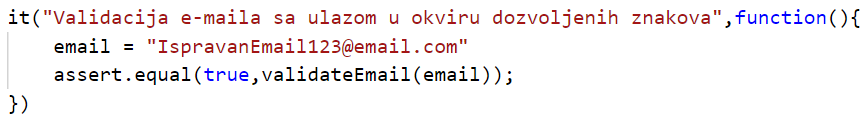
\includegraphics[width=1\linewidth]{"slike/ispravnaValidacija.png"}
					\caption{Ispravna validacija}
					\label{fig:da-val}
				\end{figure}
			

			

			\noindent \textbf {Ispitni slučaj 2: Testiranje funkcije validateEmail}\\
			\noindent \textbf {Ulaz 1:} "NeispravanEmail.com".\\
			\noindent \textbf {Ulaz 2:} "NeispravanEmail@domena".\\
			\noindent \textbf {Ulaz 3:} "NeispravanEmail@domena.a".\\
			\noindent \textbf {Ulaz 4:} "NeispravanEmail@domena.123".\\
			\noindent \textbf {Očekivani rezultati:} Funkcija vraća \textit{false} za svaki od ulaza jer su formati e-maila nedozvoljeni.\\
			\noindent \textbf {Rezultat:} Očekivani rezultat je zadovoljen. \textcolor{green}{Metoda je prošla test.}\\
			
			% TODO: \usepackage{graphicx} required
				\begin{figure}[H]
					\centering
					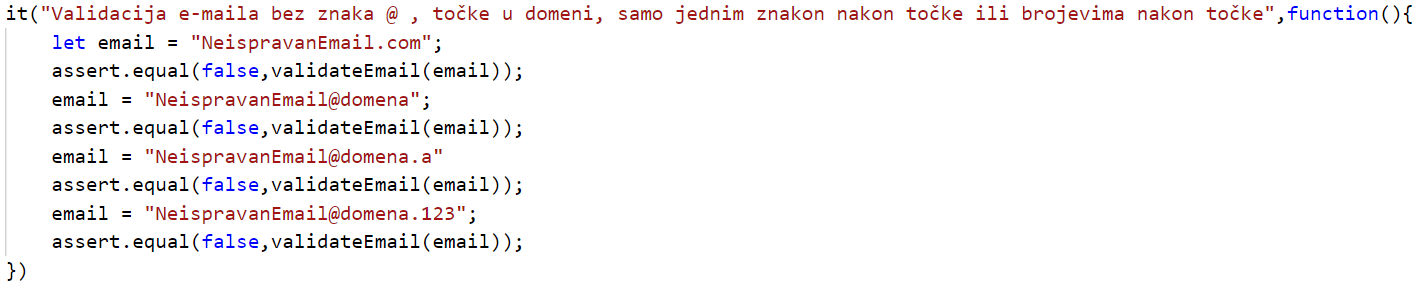
\includegraphics[width=1\linewidth]{"slike/neispravnaValidacija.png"}
					\caption{Validacija neispravno formatiranog e-maila}
					\label{fig:ne-val}
				\end{figure}
			
			\eject


			\noindent \textbf {Ispitni slučaj 3: Testiranje funkcije validateEmail}\\
			\noindent \textbf {Ulazi:} znak+"@email.com", znak = "<", ">", "(", ")", "[", "]", ".", ",", ";", ":", " ", "@", """.\\
			\noindent \textbf {Očekivani rezultat:} Funkcija vraća \textit{false} za svaki od ulaza jer je format e-mailova nedozvoljen.\\
			\noindent \textbf {Rezultat:} Očekivani rezultat je zadovoljen. \textcolor{green}{Metoda je prošla test.}\\

			% TODO: \usepackage{graphicx} required
				\begin{figure}[H]
					\centering
					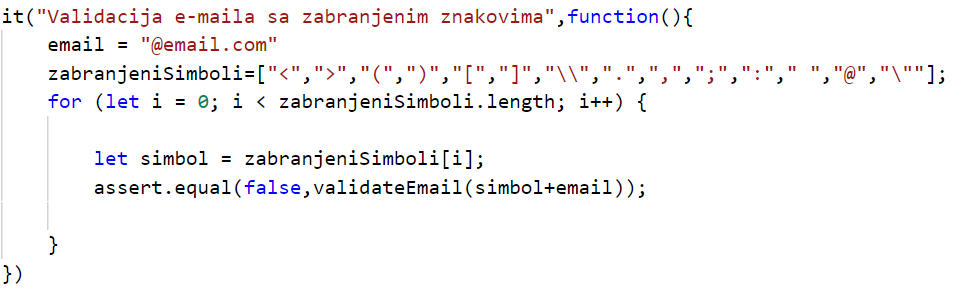
\includegraphics[width=1\linewidth]{"slike/validacijaSaZabranjenimZnakovima.png"}
					\caption{Validacija e-maila koji sadrži zabranjene znakove}
					\label{fig:zab-val}
				\end{figure}

			
			\noindent \textbf {Ispitni slučaj 4: Kalkulacija pozicije s ispravnim podacima}\\
			\noindent \textbf {Ulazi:} Podaci={"1":[10,9],"2":[12,23],"3":[6,0],"4":[2,9]}.\\
			\noindent \textbf {Očekivani rezultat:} Funkcija vraća vagon i poziciju u vagonu s najmanjim brojem ljudi ukoliko razlika putnika u ostalim vagonima nije 30 ili više.\\
			\noindent \textbf {Rezultat:} Očekivani rezultat je zadovoljen. \textcolor{green}{Metoda je prošla test.}\\

			% TODO: \usepackage{graphicx} required
				\begin{figure}[H]
					\centering
					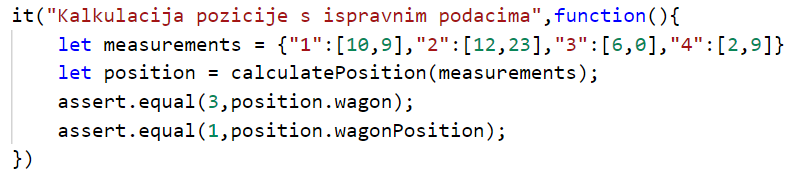
\includegraphics[width=1\linewidth]{"slike/kalkulacija1.png"}
					\caption{Kalkulacija s ispravnim podacima}
					\label{fig:isp-kal}
				\end{figure}

			\noindent \textbf {Ispitni slučaj 5: Kalkulacija pozicije s vlakom bez putnika }\\
			\noindent \textbf {Ulazi:} Podaci={"1":[0,0],"2":[0,0],"3":[0,0],"4":[0,0]}.\\
			\noindent \textbf {Očekivani rezultat:} Funkcija vraća stražnji dio prvog vagona.\\
			\noindent \textbf {Rezultat:} Očekivani rezultat je zadovoljen. \textcolor{green}{Metoda je prošla test.}\\

			% TODO: \usepackage{graphicx} required
				\begin{figure}[H]
					\centering
					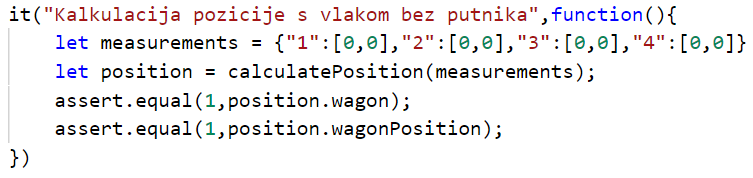
\includegraphics[width=1\linewidth]{"slike/kalkulacijaBezPutnika.png"}
					\caption{Kalkulacija bez putnika}
					\label{fig:nul-kal}
				\end{figure}
		
			\noindent \textbf {Ispitni slučaj 6: Kalkulacija pozicije s razlikom putnika većom od 30 u jednom vagonu }\\
			\noindent \textbf {Ulazi:} Podaci={"1":[0,30],"2":[20,24],"3":[15,20],"4":[18,26]}.\\
			\noindent \textbf {Očekivani rezultat:} Funkcija vraća vagon s razlikom od 30 putnika ili više.\\
			\noindent \textbf {Rezultat:} Očekivani rezultat je zadovoljen. \textcolor{green}{Metoda je prošla test.}\\

			% TODO: \usepackage{graphicx} required
				\begin{figure}[H]
					\centering
					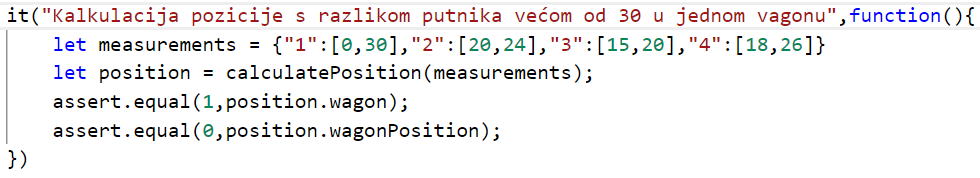
\includegraphics[width=1\linewidth]{"slike/kalkulacijaSRazlikomOd30.png"}
					\caption{Kalkulacija s razlikom od 30 putnika u jednom vagonu}
					\label{fig:j-kal}
				\end{figure}

			\noindent \textbf {Ispitni slučaj 7: Kalkulacija pozicije s razlikom putnika većom od 30 u više vagona }\\
			\noindent \textbf {Ulazi:} Podaci={"1":[0,30],"2":[60,94],"3":[31,58],"4":[50,73]}.\\
			\noindent \textbf {Očekivani rezultat:} Funkcija vraća vagon s najvećom razlikom.\\
			\noindent \textbf {Rezultat:} Očekivani rezultat je zadovoljen. \textcolor{green}{Metoda je prošla test.}\\

			% TODO: \usepackage{graphicx} required
				\begin{figure}[H]
					\centering
					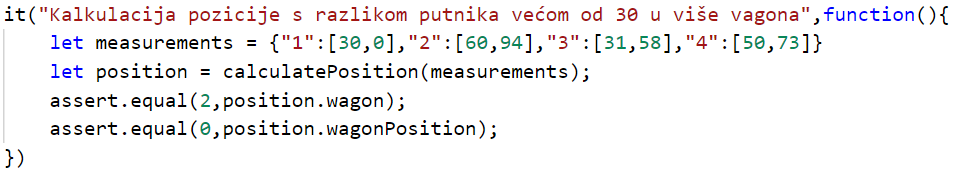
\includegraphics[width=1\linewidth]{"slike/kalkulacijaSRazlikomOd30uVise.png"}
					\caption{Kalkulacija s razlikom od 30 putnika u više vagona}
					\label{fig:v-kal}
				\end{figure}
			
			\noindent \textbf {Ispitni slučaj 8: Kalkulacija pozicije s neispravnim podacima}\\
			\noindent \textbf {Ulazi:} Podaci={"1":"Krivi podatak","2":"Krivi podatak","3":"Krivi podatak","4":"Krivi podatak"}.\\
			\noindent \textbf {Očekivani rezultat:} Funkcija izbacuje error o krivom podatku.\\
			\noindent \textbf {Rezultat:} Očekivani rezultat je zadovoljen. \textcolor{green}{Metoda je prošla test.}\\

			% TODO: \usepackage{graphicx} required
				\begin{figure}[H]
					\centering
					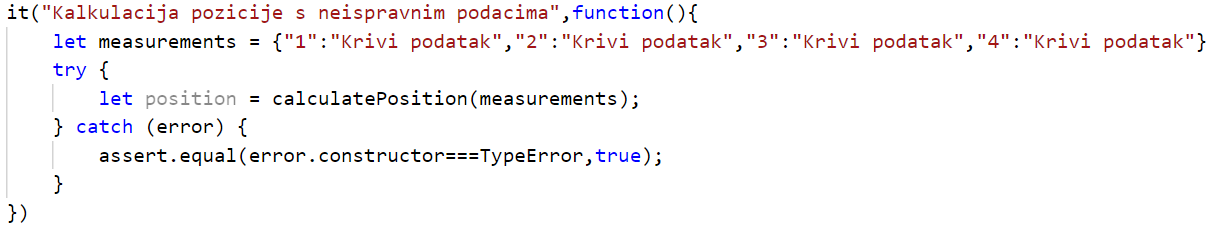
\includegraphics[width=1\linewidth]{"slike/kalkulacijaSNeispravnimPodacima.png"}
					\caption{Kalkulacija s neispravnim podacima}
					\label{fig:neisp-kal}
				\end{figure}


			% TODO: \usepackage{graphicx} required
				\begin{figure}[H]
					\centering
					
\includegraphics[width=1\linewidth]{"slike/rezultati.png"}
					\caption{Prikaz rezultata izvođenja JUnit testova u razvojnom okruženju}
					\label{fig:rez}
				\end{figure}
			
			\eject
			\subsection{Ispitivanje sustava}
			
			{Ispitivanje je provedeno pomoću Selenium IDE. Cilj je bila provjera funkcionalnosti, rubnih uvjeta i pogrešaka u sustavu. Selenium IDE je potrebno instalirati kao ekstenziju u tražilici. Zatim, nakon postavljanja URL-a testirane stranice, izvrši se test čije akcije ostaju pamćene u okviru Seleniuma i kako bi se test mogao izvršavati automatiziriano. Testovi su izvršeni na aplikaciji otvorenoj na lokalnom računalu. \hfill\break


{\noindent \textbf{\textit{Ispitni slučaj 1: Registracija}}\\
\textbf{Uvjeti}:
			 \begin{enumerate}
				\item Prilikom pokretanja testa korisnik ne smije već biti prijavljen.
				\item Korisnik mora otvoriti stranicu za registraciju na PassDirect-u.
			 \end{enumerate}
\textbf{Očekivani rezultat}: Registracija neće uspijeti za netočno potvrđenu lozinku i netočan oblik e-maila, a uspjet će ako se točno ispravi i pokuša ponovno.\\
\textbf{Tijek}:
			 \begin{enumerate}
			 	\item U polja na registracijskom obrascu uneseni su korisnički podatci s krivom potvrdom lozinke i krivim formatom e-maila.
			 	\item Odabir gumba za registraciju.
			 	\item Ispis poruke i odbijanje registracije zbog neispravnih podataka.
			 	\item Točno ispravljena potvrda lozinke.
			 	\item Ispis poruke i odbijanje registracije zbog neispravnih podataka.
			 	\item Točno ispravljen e-mail.
			 	\item Odabir gumba za registraciju.
			 	\item Prihvat registracije i prikaz početnog ekrana.
			 \end{enumerate}
			 \noindent \textbf{Rezultat}:
			 Svi očekivani rezultati su zadovoljeni. Aplikacija je prošla test. \\

\begin{lstlisting}
Running 'Registracija'
open on /login OK
click on css=.register OK
click on name=firstname OK
type on name=firstname with value Ivan OK
type on name=lastname with value Ivanic OK
type on name=email with value kriviemail@email@email.com OK
type on name=password with value Lozinka123 OK
type on name=confirmpassword with value KrivaLozinka OK
sendKeys on name=confirmpassword with value ${KEY_ENTER} OK
click on css=.app-wrapper OK
type on name=confirmpassword with value Lozinka123 OK
sendKeys on name=confirmpassword with value ${KEY_ENTER} OK
mouseDownAt on css=.app-wrapper with value 24,368 OK
mouseMoveAt on css=.app-wrapper with value 24,368 OK
mouseUpAt on css=.app-wrapper with value 24,368 OK
click on css=.app-wrapper OK
type on name=email with value dobaremail@email.com OK
sendKeys on name=email with value ${KEY_ENTER} OK
'Registracija' completed successfully
\end{lstlisting}}\hfill\break





{\noindent \textbf{\textit{Ispitni slučaj 2: Neispravna prijava}}\\
\textbf{Uvjeti}:
			 \begin{enumerate}
				\item Prilikom pokretanja testa korisnik ne smije već biti prijavljen.
				\item Korisnik mora otvoriti početnu stranicu PassDirecta(Login).
			 \end{enumerate}
\textbf{Očekivani rezultat}: Prijava u stranicu će biti odbijena zbog unosa e-maila neregistriranog korisnika.\\
\textbf{Tijek}:
			 \begin{enumerate}
			 	\item U polja na obrascu za prijavu uneseni su e-mail za koji ne postoji prijavljeni korisnik u sustavu i lozinka.
			 	\item Odabir gumba za registraciju.
			 	\item Ispis poruke i odbijanje prijave zbog neispravnih podataka.
			 \end{enumerate}
			 \noindent \textbf{Rezultat}:
			 Očekivani rezultat je zadovoljen, pošto korisnik nije ulogiran. Aplikacija je prošla test. \\


\begin{lstlisting}
Running 'Neispravna prijava'
open on /login OK
click on name=email OK
type on name=email with value kriviEmail@email.com OK
type on name=password with value Lozinka123 OK
click on css=.submit OK
mouseOver on css=.submit OK
mouseOut on css=.submit OK
'Neispravna prijava' completed successfully
\end{lstlisting}}\hfill\break





{\noindent \textbf{\textit{Ispitni slučaj 3: Prijava, pretraga voznog reda i kupnja karte}}\\
\textbf{Uvjeti}:
			 \begin{enumerate}
				\item Prilikom pokretanja testa korisnik ne smije već biti prijavljen.
				\item Korisnik mora otvoriti početnu stranicu PassDirecta(Login).
			 \end{enumerate}
\textbf{Očekivani rezultat}: Uspješna prijava u stranicu PassDirecta, pretraga voznog reda, te kupnja karte za odabranu liniju, odnosno vlak.\\
\textbf{Tijek}:
			 \begin{enumerate}
			 	\item U polja na obrascu za prijavu uneseni su e-mail i lozinka za postojećeg korisnika.
			 	\item Odabir gumba za registraciju.
			 	\item Prikaz početnog ekrana aplikacije.
				\item Odabir mjesta polaska i mjesta dolaska te datuma putovanja u zaglavlju stranice.
				\item Odabir gumba za pretraživanje voznog reda.
				\item Prikaz dostupnih linija za odabrane podatke.
				\item Odabir željene linije za koju se kupuje karta.
				\item Prikaz ekrana za checkout s već popunjenim e-mailom, imenom i prezimenom.
				\item Unos podataka o kartici.
				\item Odabir gumba za plaćanje.
				\item Prikaz obavijesti o uspješnoj transakciji.
			 \end{enumerate}
			 \noindent \textbf{Rezultat}:
			 Očekivani rezultati se zadovoljeni: nakon prijave u sustav, korisnik pretraži vozni red i kupi kartu. Aplikacija je prošla test. \\




\begin{lstlisting}
Running 'Prijava, pretraga voznog reda i kupnja karte'
open on /login OK
click on name=email OK
type on name=email with value pero@email.com OK
type on name=password with value Lozinka123 OK
sendKeys on name=password with value ${KEY_ENTER} OK
click on name=to OK
select on name=to with value label=Split OK
click on css=.right > .button OK
mouseOver on css=.right > .button OK
mouseOut on css=.right > .button OK
click on xpath=//div[@id='100']/h5/span[8]/button OK
click on id=cardNo OK
type on id=cardNo with value 1111 1111 1111 1111 OK
click on id=CVV OK
type on id=CVV with value 111 OK
click on id=expDate OK
click on id=expDate OK
click on id=expDate OK
type on id=expDate with value 0001-01 OK
type on id=expDate with value 0012-01 OK
click on css=.submit OK
click on css=.button-succesful OK
'Kupnja karte' completed successfully
\end{lstlisting}}\hfill\break






{\textbf{\textit{Ispitni slučaj 4: Prijava administratora, ispis korisnika i brisanje korisnika}}\\
\textbf{Uvjeti}:
			 \begin{enumerate}
				\item Prilikom pokretanja testa korisnik ne smije već biti prijavljen.
				\item Korisnik mora otvoriti početnu stranicu PassDirecta(Login).
				\item Korisnik prije prijave mora imati dodijeljenu rolu administratora.
				\item U bazi/sustavu mora postojati barem jedan korisnik koji.
			 \end{enumerate}
\textbf{Očekivani rezultat}: Uspješna prijava administratora u stranicu, pregled ispisa korisnika i brisanje korisničkih profila.\\
\textbf{Tijek}:
			 \begin{enumerate}
			 	\item U polja na obrascu za prijavu uneseni su e-mail i lozinka za postojećeg administratora.
			 	\item Odabir gumba za registraciju.
			 	\item Prikaz početnog ekrana aplikacije s listom korisnika.
				\item Odabir gumba za brisanje kraj jednog od korisnika.
				\item Korisnik je obrisan iz baze podataka.
				\item Prikaz osvježene liste korisnika.
			 \end{enumerate}
			 \noindent \textbf{Rezultat}:
			 Očekivani rezultati se zadovoljeni: nakon prijave u sustav, administrator pregleda i izbriše korisnika. Aplikacija je prošla test. \\



\begin{lstlisting}
Running 'Prijava administratora,ispis korisnika i brisanje profila'
open on /login OK
click on name=email OK
type on name=email with value admin@email.com OK
type on name=password with value Lozinka123 OK
sendKeys on name=password with value ${KEY_ENTER} OK
click on css=#korisnik1\@email\.com span:nth-child(5) > .buttonAH OK
'Prijava administratora,ispis korisnika i brisanje profila' completed 
successfully
\end{lstlisting}
 }}
	
 
 
	
			
			\eject 
		
		
		\section{Dijagram razmještaja}
			
			{Dijagram razmještaja statički opisuje topologiju sustava s fokusom na odnos skopovlja i programskog dijela projekta. Organizacija sustava se zasniva na arhitekturi klijent - poslužitelj. Klijent na svome računalu koristi web preglednik kako bi pristupio aplikaciji koja se nalazi na Heroku servisu. Više korisnika može pristupiti aplikaciji, putem HTTP veze. Heroku web server sadrži web poslužitelj i poslužitelj baze podataka na kojima se nalaze sama aplikacija, odnosno baza podataka aplikacije. }
				
			 % TODO: \usepackage{graphicx} required
				\begin{figure}[H]
					\centering
					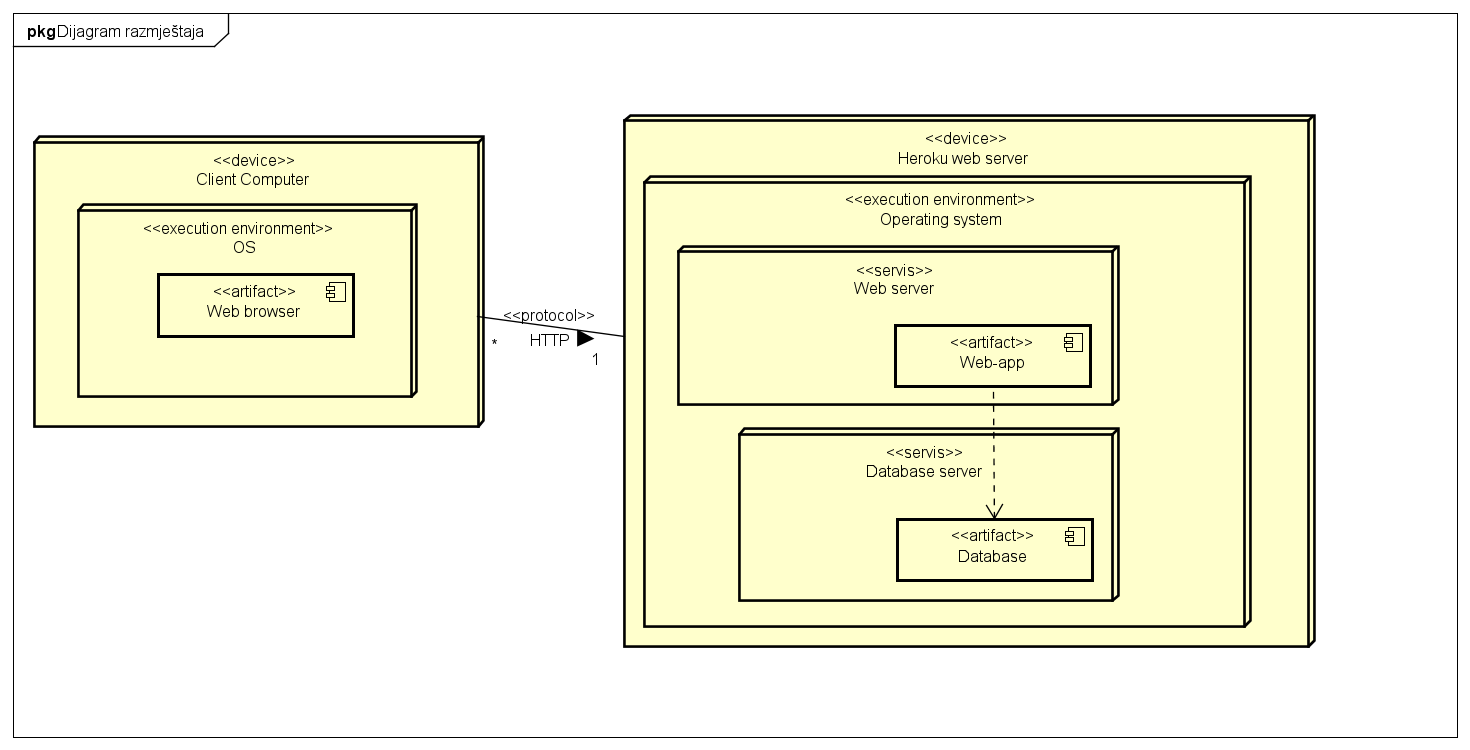
\includegraphics[width=1\linewidth]{"slike/specDiagram.png"}
					\caption{Dijagram razmještaja}
					\label{fig:dij-raz}
				\end{figure}
			
			\eject 
		
		\section{Upute za puštanje u pogon}
		
			 {U ovom poglavlju opisano je puštanje aplikacije u pogon. Puštanje je izvedeno uz pomoć platforme Heroku. 
%TODO: \usepackage{graphicx} required
				\begin{figure}[H]
					\centering
					
\includegraphics[width=1\linewidth]{"slike/herokuPocetna.png"}
					\caption{Platforma Heroku}
				\end{figure}
			
			
Najprije je potrebno registrirati račun te se prijaviti. Nakon prijave korisniku je otvorena stranica sa postojećim aplikacijama te opcijom za stvaranje nove. 
%TODO: \usepackage{graphicx} required
				\begin{figure}[H]
					\centering
					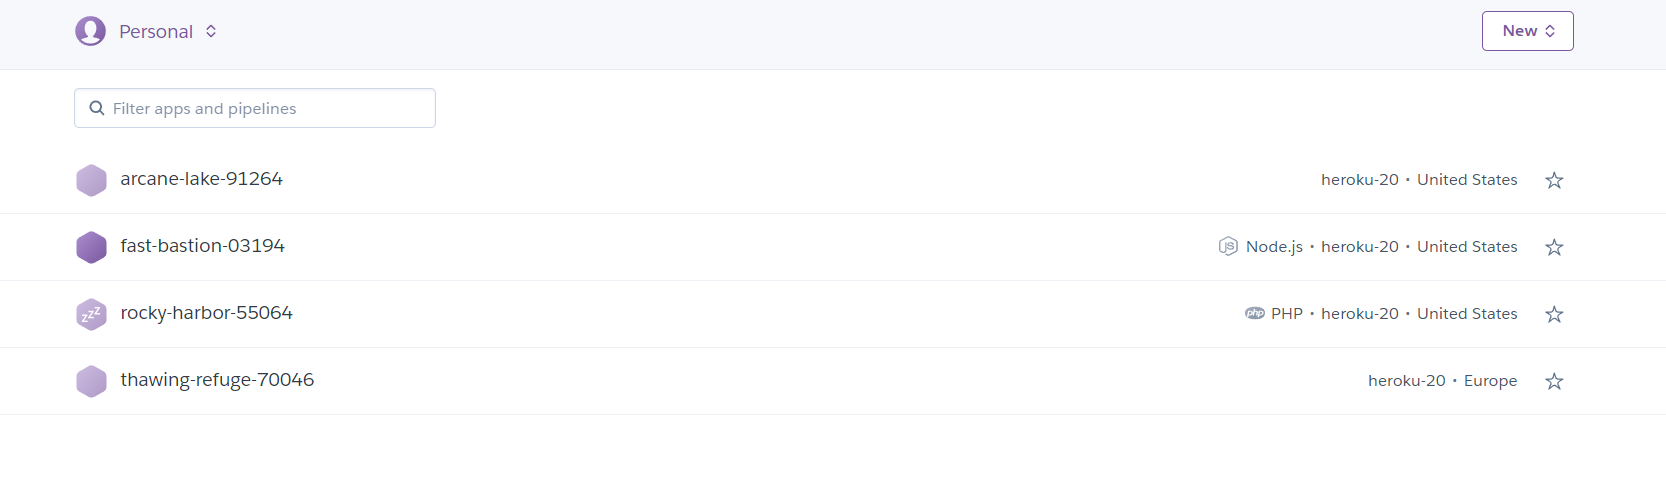
\includegraphics[width=1\linewidth]{"slike/herokuNewApp.png"}
					\caption{1. korak: "New"}
				\end{figure}
\eject			
			
 Odabirom gumba za stvaranje nove aplikacije otvara se obrazac za popunjavanje polja za osnovne informacije o aplikaciji (naziv i regija).
%TODO: \usepackage{graphicx} required
				\begin{figure}[H]
					\centering
					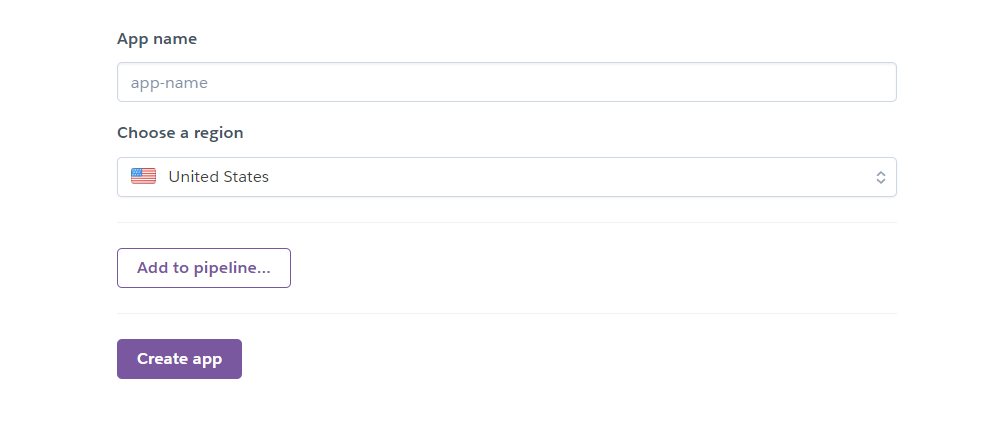
\includegraphics[width=1\linewidth]{"slike/herokuNew.png"}
					\caption{2. korak: Obrazac}
				\end{figure}						
			
Nakon što su je Heroku platformi napravljena i postavljena aplikacija, još je preostao upload izvornog koda uz pomoć HerokuCLI. U terminalu na računalu se pozicionira u direktorij IzvorniKod i unese se naredba za login u heroku:
\newline - heroku login \newline
Sada moramo izvesti sljedeće naredbe kako bismo postavili aplikaciju na Heroku:
\newline  - cd ../izvorniKod 
\newline - heroku git: remote -a naziv-aplikacije-na-heroku
\newline - git add .
\newline - git commit -m "Commit"
\newline - git push heroku master \newline
\textbf{Kreiranje baze podataka}\\
{U ormconfig.json datoteci su nam zapisani podaci za povezivanje i kreiranje baze podataka kako je prikazano na slici ispod. 
%TODO: \usepackage{graphicx} required
				\begin{figure}[H]
					\centering
					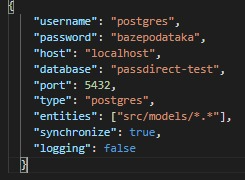
\includegraphics[width=0.6\linewidth]{"slike/inicijalizacijaBP.png"}
					\caption{Kreiranje baze podataka}
				\end{figure}			
Kako bismo imali kontrolu nad našom bazom podataka koja se sada nalazi na herokuovom serveru, za naš heroku projekt dodajemo Heroku Postgres plugin. Ovaj plugin nam omogućuje da se premjestimo u psql CLI te otud koristeći SQL upite kontroliramo i izmjenjujemo stanje BP. Kako bismo pokrenuli CLI potrebno je u terminalu računala na kojem radimo upisati naredbu: heroku pg:psql --app pass-direct
}		
}
			
			
			
			\eject 